\chapter{Prototipo 4: Desarrollo de un sistema híbrido de recomendación de platillos}
  \section{Análisis}
    \subsection{Objetivo}
      Desarrollar un sistema híbrido para la recomendación de platillos que conlleve la demostración de la funcionalidad proporcionada por el API en un caso de estudio particular.

    \subsection{Características}
    \begin{itemize}
      \item El sistema permitirá realizar recomendaciones de platillos de acuerdo a sus características de los mismos (basadas en contenido).
      \item El sistema permitirá realizar recomendaciones de platillos con base en la interacción de los usuarios finales a través de ratings o evaluaciones cuantitativas (por filtrado colaborativo).
      \item El sistema permitirá el registro de usuarios finales, así como su autenticación para el uso de las funcionalidades del sistema.
      \item El sistema permitirá la visualización de los platillos a los usuarios no registrados.
      \item El sistema permitirá la recomendación para los usuarios no registrados a través del manejo de cookies en el navegdor y su interacción con los platillos.
    \end{itemize}

    \subsection{Restricciones}
    \begin{itemize}
      \item El sistema se verá limitado a las características y cantidad de platillos registrados para realizar las recomendaciones.
      \item El sistema no permitirá el registro de platillos a usuarios no registrados.
    \end{itemize}

    % Insertar historias de usuario aqui

  \section{Diseño}

    Para desarrollar las características mencionadas previamente, se debe tomar en cuenta el modelo de datos propio del caso de estudio que podemos observar en la figura ~\ref{fig:model_cs}

    \begin{landscape}
      \begin{figure}[h!]
        \centering
        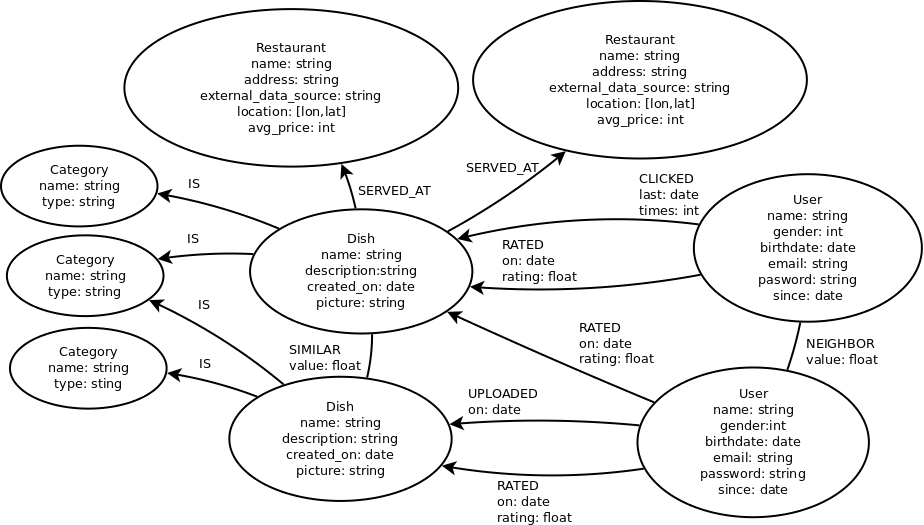
\includegraphics[width=25cm]{./images/sc_data_model}
        \caption{Modelo de datos del caso de estudio}
        \label{fig:model_cs}
      \end{figure}
    \end{landscape}

  El diseño de las clases creadas  a partir del modelo de datos propuesto: User, Dish, Characteristic y Restaurant, así como sus relaciones producto de la interacción entre ellos: Affinity, Neighbor, Upload, Click y Rate, permiten aunado a la funcionalidad propia del API realizar el conjunto de recomendaciones de acuerdo a las necesidades del sistema. Para esto, se desarrollaron un conjunto de clases para exponer, a través de servicios web, las operaciones básicas de un CRUD de las clases de dominio; así como para la creación de las posibles relaciones existentes entre estas entidades y las recomendaciónes generadas por la API.

  Para el desarrollo de los servicios web se toma en cuenta lo siguiente:
  \begin{itemize}
    \item Un contenedor llamado \"rest\". Este contenedor contendrá todos los servicios web que son expuestos para consumirlos en el caso de estudio.
    \item Los recursos. Estos recursos son las clases que hacen referencia a cada entidad del caso de estudio. El nombre del mismo está expresado por el nombre de la clase de dominio a la que hace referencia concatenado con la palaba \"ws\".
    \item El conjunto de métodos que contienen las clases de los servicios web. Es decir, cada uno de los recursos contendrá métodos que manejan las operaciones básicas CRUD (Create, Retrieve, Update, Delete y RetrieveAll) para la creación de las entidades de dominio; métodos para la creación de las relaciones existentes entre estas para la generación de las recomendaciones por parte de la API. Y finalmente, se exponen las recomendaciones obtenidas, para que, en conjunto con el caso de estudio, se tenga una mejor apreciación de la funcionalidad de esta API.
    \item Se declara el tipo de respuesta que dan estos servicios y el tipo . Debe ser un formato válido para cualquier dispositivo que consuma estos servicos. El tipo propuesto para este caso de estudio es un JSON válido y bien formado.
  \end{itemize}

  \section{Resultados}
    Utilizando el comportamiento de la API como parte de la funcionalidad del sistema, integrado con las clases de dominio y los servicios diseñados previamente obtenemos la estructura mostrada en el diagrama de clases de la figura~\ref{fig:monster_classes}. 

    \begin{landscape}
      \begin{figure}[h!]
        \centering
        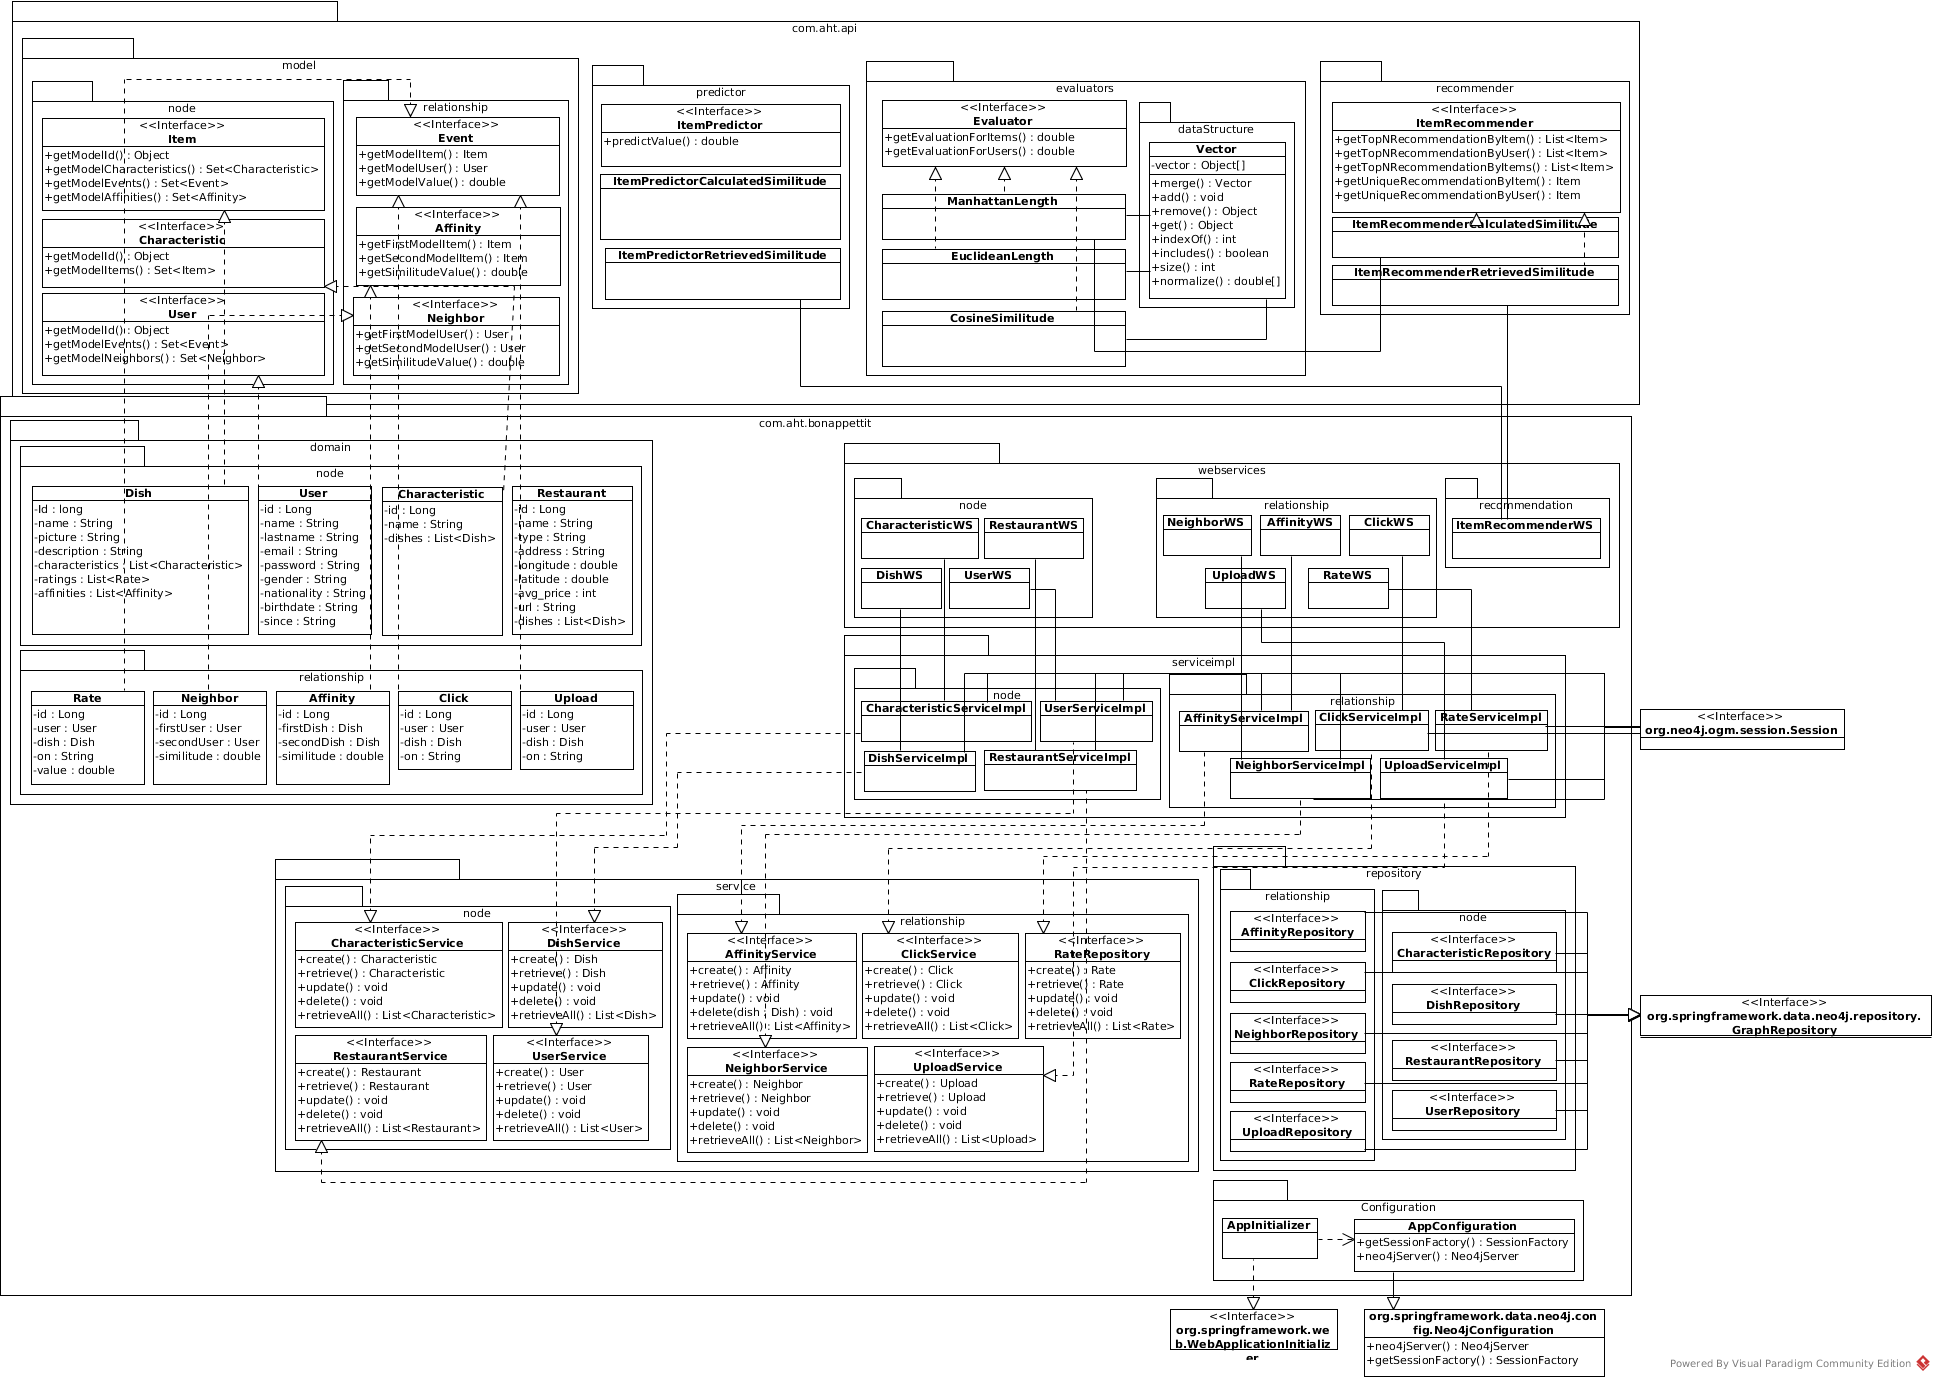
\includegraphics[width=25cm]{./images/monster_class}
        \caption{Diagrama de clases del prototipo 4}
        \label{fig:monster_classes}
      \end{figure}
    \end{landscape}

    Así finalmente se desarrolla el sistema web del caso de estudio, consumiendo los servicios web proporcionados por el back-end del sistema en una aplicación desarrollada con Angular.js, que a través de servicios y controladores que siguen el patrón MVC, permiten mostrar los datos en una interfaz gráfica al usuario final acorde a las características necesarias, como la mostrada en la figura~\ref{fig:final_bonappettit}


      \begin{figure}[h!]
        \centering
        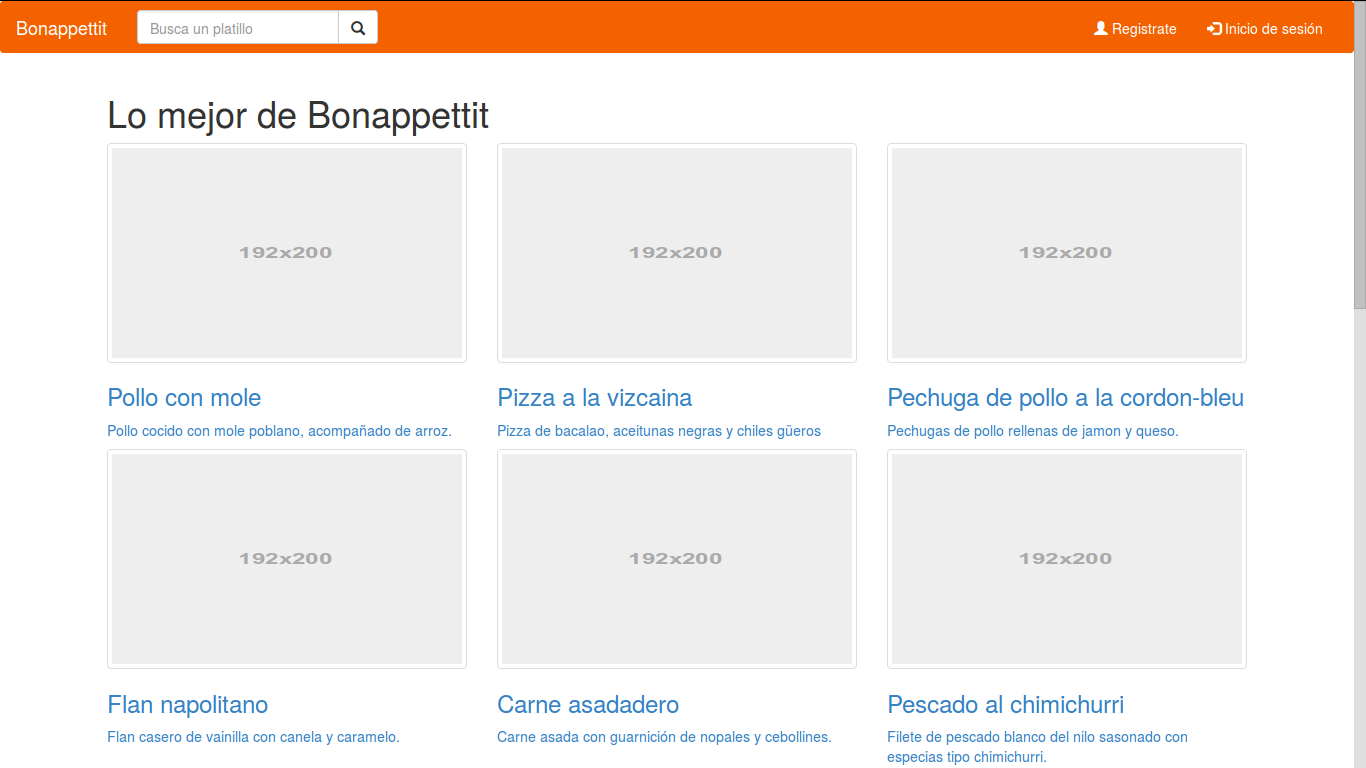
\includegraphics[width=16cm]{./images/p4_bonappettit}
        \caption{Interfaz gráfica del sistema}
        \label{fig:final_bonappettit}
      \end{figure}

